\documentclass[../main/main.tex]{subfiles}

\newdate{date}{11}{06}{2020}

\begin{document}

\section{Lecture 23}
 \displaydate{date}. Compiled:  \today. Martina 

\subsubsection{Slide 394}

\begin{figure}[h!]
\centering
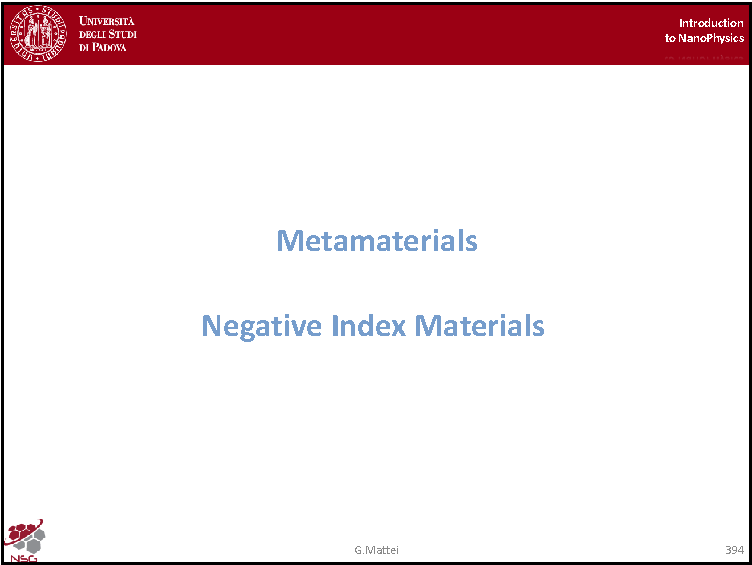
\includegraphics[page=1,width=0.9\textwidth]{../lessons/pdf_file/23_lesson.pdf}
\end{figure}

In this lesson we will speak about a vast class of materials which can be called metamaterials. In this way we label the materials which are made by combining properties of different materials to create a novel material whose properties are not simply the sum of the properties of the individual components but you can obtain novel functionalities and we will see some class of metamaterials which are the so called "negative refractive index materials", which are a quite peculiar kind of materials exhibiting apparently strange properties but which can be demonstrated to be real.

As I mentioned several times during this course, the concept of metamaterial is a sort of unifying concept and all the systems that we have seen can be considered metamaterials. Of course there are special classes in which this concept comes out in a more profound way and we will try to deal with such kind of systems.

\newpage

\subsubsection{Slide 395}

\begin{figure}[h!]
\centering
\includegraphics[page=2,width=0.9\textwidth]{../lessons/pdf_file/23_lesson.pdf}
\end{figure}

To start the discussion I would like to highlight this paper published by Victor Veselago in 1968 which received large attention at that time but it was rediscovered several years later as a very interesting source of information for developing the concept of negative refractive index materials. 

The paper was on the electrodynamics of substances with simultaneously negative values of $\epsilon$ and $\mu$ and in this paper he analyzes the possibility to investigate the electrodynamical properties of materials in which for some specific frequencies they are both negative.

The anomalies of this kind of materials come from the usual consideration that we use for the solution of the Maxwell equations. When we relate the $k$ vector of the planar wave that we want to propagate in our system to the wave in vacuum, that is, normally we relate them through the refractive index squared or through the concept of dielectric function of the material, and normally this is true when we are considering non magnetic system in which we can assume $\mu = 1$ so that this equation holds, but in general we have to deduce the more general equation in which $n^2$ is related to the product of $\epsilon$ and $\mu$. 

Supposing that $\epsilon$ and $\mu$ are real numbers (functions), in the sense that they belong to non dissipative materials, this implies that we can satisfy this equation either when $\epsilon$ and $\mu$ are positive, which is the simplest solution, but also when they are negative, so that their product is positive, and in this case we can obtain a real refractive index with no absorption. So the possibilities that Veselago discussed are 3. 

The first instance is the properties of materials unaffected by the simultaneous change of sign; the second possibility is that having both $\epsilon$ and $\mu$ negative may contradict some natural law, and the last possibility is that the substances with both negative $\epsilon$ and $\mu$ may exist but with different properties with respect to their counterpart with $\epsilon$ and $\mu$ positive. 

The real answer is that in general in nature we have materials with $\epsilon$ and $\mu$ which are negative, but not in general simultaneously, so in order to achieve this property we need to have a metamaterial, that is a material which we build on purpose to obtain such functionality. 

\newpage

\subsubsection{Slide 396}

\begin{figure}[h!]
\centering
\includegraphics[page=3,width=0.9\textwidth]{../lessons/pdf_file/23_lesson.pdf}
\end{figure}

Of course the starting point of Veselago analysis are Maxwell equations as we have seen several times during this course, but now we want to empathize not the general properties but some specific properties of these equations.  

\newpage

\subsubsection{Slide 397}

\begin{figure}[h!]
\centering
\includegraphics[page=4,width=0.9\textwidth]{../lessons/pdf_file/23_lesson.pdf}
\end{figure}

They are summarized in this sentence taken from the paper in which Veselago stands the interest for having both $\epsilon$ and $\mu$ less than zero in respect of the fact that such materials can exist or not. 

So Veselago describes the problem in a very general way. The concept that we can use to describe the problem is the so called Rightness, that is the relative orientation of the electric and magnetic field and the wave vector in the solution of the Maxwell equations.

You may remember that if we search for a plane wave solution of the Maxwell equations, the nabla operator is equivalent to a multiplicative operator $i\mathbf{k}$ and the temporal derivative is equivalent to a multiplicative operator $-i\omega$. If we use this analogy we can recast the first equation and write it as follows.

The energy flow in the system is controlled by the Poynting vector which is defined as the vector product between the electric and magnetic field. 

\newpage

\subsubsection{Slide 398}

\begin{figure}[h!]
\centering
\includegraphics[page=5,width=0.9\textwidth]{../lessons/pdf_file/23_lesson.pdf}
\end{figure}

If we look at the relative orientation of this three vectors $\mathbf{E, H}$ and $\mathbf{S}$ or $\mathbf{k}$, we can understand the concept of Rightness or handedness in the interpretation of the solution according to the algebraic sign of $\epsilon$ and $\mu$. 

Suppose that $\epsilon$ and $\mu$ are both positive, for instance this is the simplest case; of course the first equation tells us that this factor here is positive, so $\mathbf{k} \times \mathbf{E}$ is equal something proportional to $\mathbf{H}$, so in this case $\mathbf{E, H}$ and $\mathbf{k}$ constitute a right-handed triplet of vectors, in the typical way, and consistently $\mathbf{k} \times \mathbf{H}$ is minus a constant times $\mathbf{E}$. So the geometrical situation of the three vectors is for instance with $\mathbf{E}$ on the $x$ axis, $\mathbf{H}$ on the $y$ aixis and $\mathbf{k}$ on the $z$ axis. 

If we take the vector product of $\mathbf{E}$ and $\mathbf{H}$ we see that this is the normal discussion of Maxwell equations, as it is parallel and aligned with $\mathbf{k}$, so even $\mathbf{S}$ is on the $z$ axis, that is the scalar product between $\mathbf{S}$ and $\mathbf{k}$ is 0 because they are aligned on the same vector.

On the contrary if we switch the sign simultaneously of $\epsilon$ and $\mu$ what we obtain is that now $\mathbf{E}$, $\mathbf{H}$ and $\mathbf{k}$ constitute a left-handed triplet, because if we change the sign here we have the $\mathbf{H}$ vector in the opposite direction with respect to the previous one, so that this is consistent if we change the sign of $\epsilon$. 

So in this case we can use the left-handed to recover the alignment of $\mathbf{E}$, $\mathbf{H}$ and $\mathbf{k}$, but in this case if we calculate the Poynting vector which involves the two changes of the algebraic sign, in this case it is in the opposite $z$ direction if we are considering the left-handed triplet.

So $\mathbf{E}$, $\mathbf{H}$ and $\mathbf{k}$ are left-handed triplet but $\mathbf{E}$, $\mathbf{H}$ and $\mathbf{S}$ are standard right-handed triplet, so in this case the scalar product of $\mathbf{S}$ and $\mathbf{k}$ is less than zero and we have the apparent counterintuitive situation in which the energy flows in the opposite direction as the propagation of the wave which is quite unusual expectation.

\newpage

\subsubsection{Slide 399}

\begin{figure}[h!]
\centering
\includegraphics[page=6,width=0.9\textwidth]{../lessons/pdf_file/23_lesson.pdf}
\end{figure}

We can define the phase velocity as usual as $\frac{\omega}{k}$, and a group velocity which counts the energy and the information in the system which is the gradient with respect to $\mathbf{k}$ of $\omega$ and of course this two velocities are opposite in  the case of left-handed material because the different orientation, the two handedness, of the three vectors. 

We can recast in a more formal way the definition of the direction cosines for the three vectors $\mathbf{E}$, $\mathbf{H}$ and $\mathbf{k}$ with this matrix $\mathbf{G}$ whose determinant is of course $p$ which is $1$ for the typical RH materials and $-1$ for LH materials. This is a useful synthetic notation for speaking about right-handed or left-handed materials. 

\newpage

\subsubsection{Slide 400}

\begin{figure}[h!]
\centering
\includegraphics[page=7,width=0.9\textwidth]{../lessons/pdf_file/23_lesson.pdf}
\end{figure}

If we use this notation to describe a very simple phenomenon in standard optics, that is refraction at an interface, we obtain a very interesting result in this case. 

If we analyze the Snell law, suppose that we have an interface between a material, it could be air or whatever you want, and a normal material (glass, dielectric), so if we enter with $\mathbf{k}$ forming a given angle with respect to the normal to the interface, we can decompose for instance the electric field which is perpendicular to this $\mathbf{k}$ vector in the tangential and normal component, and the Poynting vector is aligned with $\mathbf{k_1}$.

Upon reflection of course we need to apply the continuity equation at the interface, so the tangential component of the electric field is conserved for instance whereas the normal component of the electric field is changed because is the  normal component of the displacement field that is conserved, that is $\epsilon_1$ times the normal component of the electric field is conserved. 

So if $\epsilon_2$ is larger with respect to the first one, this is normally the case, the component of the electric field should be decreased with respect to the previous value, and so the resulting vector $\mathbf{E_2}$ in the new material is directed in another way with respect to the incoming electric field, and since $\mathbf{k_2}$ should be perpendicular to that value of the electric field, the light should bend in this case toward the normal to the interface, and also $\mathbf{S_2}$ is directed in the same direction. This is the standard Snell law we are familiar with.

\newpage

\subsubsection{Slide 401}

\begin{figure}[h!]
\centering
\includegraphics[page=8,width=0.9\textwidth]{../lessons/pdf_file/23_lesson.pdf}
\end{figure}

Suppose now that we have a metamaterial in which we can switch the sign of $\epsilon_2$ and $\mu_2$; the net result is that now the sign of the normal component of the field is reversed in the sense that is shrinked and reversed with respect to the previous situation, and in this case the resulting vector, since the tangential component in unaffected because this equation does not involve $\epsilon$, we will end up in the situation in which $\mathbf{E}$ is now in this direction here and this means that $\mathbf{k_2}$ should be perpendicular to that but directed in the opposite way with respect to the previous, so we have the strange situation in which the propagation vector $\mathbf{k_2}$ is in this direction but the $\mathbf{S_2}$ is in the direction that we expected, that is the information propagates away from the source of the light.

So, in this case we have an important information in which we have what is called negative refraction, that is the light is refracted at an angle which is exactly in modulus the previous of the Snell law but with a negative algebraic sign and moreover the phase velocity is apparently in the opposite direction with respect to the Poynting vector propagation.

\newpage

\subsubsection{Slide 402}

\begin{figure}[h!]
\centering
\includegraphics[page=9,width=0.9\textwidth]{../lessons/pdf_file/23_lesson.pdf}
\end{figure}

So if we reanalyze the entire generalized Snell law with this result, we have the incident beam and the reflected beam at the same angle that is the standard way, then we have the transmitted and refracted for RH materials in the standard way but in the LH materials in this new negative refraction condition and we can recast the generalized Snell law by using the determinant of the handedness materials 1 and 2 and the product of $\epsilon_2$ and $\mu_2$ and $\epsilon_1$ and $\mu_1$.

This is a very simple way to understand that everything is changing when we have negative refractive materials and we can recast this result telling that the refractive index is negative in the sense that we can see here with this simple algebraic manipulation.

In normal RH materials $n$ is the square root of the product $\mu \epsilon$ and we can recast this equation if $\mu$ and $\epsilon$ can be considered as two numbers $a$ and $b$. For LH materials the same definition holds but now we can change the phase of those  numbers and we can introduce this complex number which is nothing but $-1$ and in this case we have this coefficient so that we can change the sign of $a$ and $b$ simultaneously. 

In the end what we obtain is that we can factorize this phase terms, we have still the product $ab$ and then we have $e^{\frac{i \pi}{2}}$ that is again $e^{i \pi}$, so that we end up in a situation in which we can change the sign to the entire value of the square root and so in LH cases we have minus the refractive index of the corresponding RH materials with the same $\mu$ and $\epsilon$ but with opposite signs.

\newpage

\subsubsection{Slide 404}

\begin{figure}[h!]
\centering
\includegraphics[page=10,width=0.9\textwidth]{../lessons/pdf_file/23_lesson.pdf}
\end{figure}

This concept of negative refraction can be summarized in this generalized Snell law in which we have the $k_{in}$ and the $k_{refracted}$ which is now in the opposite direction, but the energy flux still goes in the right direction, the parallel component of k is preserved and also causality is preserved, because the energy is carried away from the source, that is there is no effect which occurs earlier than the cause that produces that specific effect. But of course in this case the energy goes in the right direction while the phase fronts travel in the opposite direction with respect to the energy in our system.

\newpage

\subsubsection{Slide 405}

\begin{figure}[h!]
\centering
\includegraphics[page=11,width=0.9\textwidth]{../lessons/pdf_file/23_lesson.pdf}
\end{figure}

Veselago now analyzes the effect of having a LH material combining it with RH materials and the first application that he discussed is the perfect lensing, that is if we have a stuck of RH material, LH material and RH material which could be the same as before.

The negative refraction implies that if we have a point source A in the RH material, the rays which are refracted at the LH material (in this case for instance we suppose that the LH material is the symmetric of the RH material) we have the fact that the point source A is refocused on the point B in a perfect way, that is without problem of aberration due to round refraction and with perfect correspondence between an image point with the source point.

Normally in a standard aberrated system we have that the source point A is mapped confusedly, in this case we have perfect resolution because we have sharp interfaces and not curved surfaces, so that we can have perfect reconstruction of all the rays emitted by A into the point B at this specific distance from the source. 

So, in this case the $\mathbf{S}$ propagation is indicated in this plot which fulfill causality perfectly. 

\newpage

\subsubsection{Slide 408}

\begin{figure}[h!]
\centering
\includegraphics[page=12,width=0.9\textwidth]{../lessons/pdf_file/23_lesson.pdf}
\end{figure}

Another fancy effect of LH is that if we were able to build conventional lenses with LH material we should have the opposite behaviour as in standard lenses. Normally this is a convergent lens for RH materials but in this case with LH materials this would be divergent lens. On the contrary this is a normally divergent lens and with LH materials it is a convergent lens. So these are counterintuitive properties obtained by changing the handedness of the material.

\newpage

\subsubsection{Slide 409}

\begin{figure}[h!]
\centering
\includegraphics[page=13,width=0.9\textwidth]{../lessons/pdf_file/23_lesson.pdf}
\end{figure}

It is interesting to see the effect in the real world of this change of handedness. For instance this is a ray tracing of a glass containing water and this stick is immersed into it and apparently the stick is broken at the surface due to refraction, but if instead of water with 1.33 refractive index we suppose to have water with negative refractive index of -1.33, which is something which resembles this, the bar is broken and directed in the opposite direction. 

We cans see a simulation here obtained by finite element calculation in which we compare the situation in which we enter from air into a RH material first and we have the interface with $\epsilon$ which is 1.2, so slightly different with respect to that of air, and $\mu = 1$, and in this case we have a LH material in which $\epsilon$ is -1.2 and $\mu$ is -1.

You see this is the component of the displacement field, the incoming beam is entering at a given angle with respect to the normal, so we can better appreciate the phase, and if we look at the refracted beam here we see that we have redirection in the opposite side of the normal with respect to the interface and moreover the apparent phase velocity is in the opposite direction in the two cases. 

We can see it by this simulation, and in the normal  material we have standard refraction whereas in the LH material we have an apparent wave which goes in the direction of the interface, but of course this fulfill perfectly the causality because the $\mathbf{S}$ vector goes in the expected direction with this way from the source.

\newpage

\subsubsection{Slide 410}

\begin{figure}[h!]
\centering
\includegraphics[page=14,width=0.9\textwidth]{../lessons/pdf_file/23_lesson.pdf}
\end{figure}

Another interesting effect is the reversed Doppler effect, which you may remember is the change of frequency when there is relative motion between the source and the receiver of the wave.

Whit a RH material we have the standard results for which if the source is stationary fixed and the receiver is moving either toward or far from the source, the equation can be calculated straightforwardly if we use the generalized version of the Doppler effect calculated by Veselago.

We suppose that $v_A$ is zero, the source is stationary, $v_B$ is the velocity of the receiver and we suppose that it is negative if B is moving toward A because is against the $x$ axis in this case, so that we have $\omega_0$, the emitted frequency, times $1-p$, the handedness of the material in which we are, times the velocity of the receiver $v_B$ divided by the velocity $u_S$ of the energy flux, for instance in our case the velocity of the speed of light.

If $v_B$ is negative normally we obtain an increasing in frequency, but of course if $p$ is negative because the material is LH, we still have a decrease in frequency, which is exactly the opposite that we have for normal material, that is a quite fancy result.

\newpage

\subsubsection{Slide 411}

\begin{figure}[h!]
\centering
\includegraphics[page=15,width=0.9\textwidth]{../lessons/pdf_file/23_lesson.pdf}
\end{figure}

In general we can classify materials according to the value of $\epsilon$ and $\mu$ in four different quadrants in our plane. If we have standard materials typically we are in this region here in which both are positive, we have for instance dielectrics with both $\epsilon$ and $\mu$ greater than 1 and those are double positive situation in which both are positive.

In this quadrant here we have negative $\epsilon$ and positive $\mu$ and we have for instance evanescent propagation in which the field is dumped when entering the materials (metals are in this situation at optical frequency).

The counterpart in the fourth quadrant, it is also evanescent for natural magnetic materials in which we have positive $\epsilon$ and negative $\mu$. 

The last quadrant here is when we have both negative $\epsilon$ and $\mu$, in which we have the metamaterials in which we should obtain again a behaviour symmetric of this one, that is we should have propagating signal because we do not have dumping or extinction of the beam propagating in that specific materials, because we recover exactly the same properties in terms of the refractive index of the previous situation.

We can say that this quadrant here we have positive phases and in this quadrant here negative phases or forward and backward waves in terms of the phase velocities. 

\newpage

\subsubsection{Slide 412}

\begin{figure}[h!]
\centering
\includegraphics[page=16,width=0.9\textwidth]{../lessons/pdf_file/23_lesson.pdf}
\end{figure}

Which class of materials can fulfill this rules? 

In the first quadrant we have the so called positive refraction material, double positive materials which are typically dielectrics, and in the second quadrant we have materials with absorption and with $\epsilon$ which is negative and $\mu$ which is positive, for instance metals or plasma or electrons are in this situation; we have double negative materials which are not found in nature which produce negative refraction, but we will see how to obtain them in an artificial way, and in the last quadrant we have magnetic negative component with $\epsilon$ positive, the so called Gyrotropic materials, in which we have absorption exactly for the magnetic counterpart as we have seen before for metals.

\newpage

\subsubsection{Slide 413}

\begin{figure}[h!]
\centering
\includegraphics[page=17,width=0.9\textwidth]{../lessons/pdf_file/23_lesson.pdf}
\end{figure}

The challenges of obtaining metamaterials is in engineering the $\epsilon$ and $\mu$ properties of that specific materials. Obtaining $\epsilon$ less than zero is straightforward in optical frequency, we have seen several times that any metal exhibit this property but at the same time metals do not exhibit $\mu$ less than zero, so we need to build metamaterials to obtain this effect. 

The idea is to build something which resembles atoms in which we have circulating currents due to the electrons which produce magnetic moment, so that we can construct artificially units whose size should be much less than the wavelength at which we want to operate and which produce a magnetic response.

They can be made out of non magnetic materials, a coil of copper in which circulating currents will produce magnetic field even if copper does not exhibit a strong magnetic behaviour, so that we can use this concept of localized currents induced by the incident radiation in order to circulate current in loops and possibly we can take advantage of resonant behaviour for the interaction of light with this specific materials, to get the strongest magnetic response.

Such class of materials are called resonant metamaterials because their properties can be adjusted by adjusting the geometry of artificial units in order to match a specific resonance.

\newpage

\subsubsection{Slide 414}

\begin{figure}[h!]
\centering
\includegraphics[page=18,width=0.9\textwidth]{../lessons/pdf_file/23_lesson.pdf}
\end{figure}

The typical example of this are the Split ring resonators (SRR); they are rings in which we have a split in order to obtain an equivalent circuit which is nothing but a plate capacitor and a magnetic coil in the entire range of the ring; since we are dealing with alternate current produced by the electromagnetic field there is no problem if we have a broken circuit. The equivalent circuit is that of a capacitor in series pumped by the external light.

The split ring resonator have resonance, this is a LC circuit, the geometrical link between the capacitance and the inductance are reported in this equation, where we can arrange properly the geometry of our splitting resonator, that is the thickness $d$, the opening of the split $a$, the lateral side $w$ of this square split ring, and $a$ is also the thickness of the material, so we can obtain a capacitance which is proportional to $d$ and an induction which is proportional to $\frac{w^2}{d}$, so if you remember the resonant frequency of that circuit, it is $\omega_{LC}$ which is one over the square root of LC and so we can straightforwardly see that is inversely proportional to $w$, so to the side of the split ring, so the frequency can be controlled by controlling the size of our split ring resonator.

\newpage

\subsubsection{Slide 415}

\begin{figure}[h!]
\centering
\includegraphics[page=19,width=0.9\textwidth]{../lessons/pdf_file/23_lesson.pdf}
\end{figure}

If you want to calculate explicitly the physical quantities involved in that, the induced potential difference can be calculated by the Faraday law and the resonance is the one which maximizes the current circulating in the loop, which is obtained of course when we have a minimum in the impedance $Z$ of the materials.

If we do not have any resistance we have just an LC circuit, of course we should have some resistance, so it is important to add also the $R$ in the full equation, but we want to search a resonance in the current which maximizes the magnetic dipole moment $m$ in terms of the circulating current $I$ times the area of the loop $A_{loop}$, that is the area of the split ring. 
We will get this maximum $I$ at $\omega_{LC}$, so the equivalent wavelength at which we can work is $\frac{2 \pi c}{\omega_{LC}}$, which is again linked linearly with the size of the split ring, for instance if we operate with the system in air with this $\epsilon = 1$, the split ring will resonate at a frequency $\lambda$ which is $600 nm$ with a size of the split ring of $100 nm$, so that this is simple example of split ring resonators which should operate in the visible.

The problem is that in the visible we are not able to obtain a controlled way in which we can obtain both the effective medium for the entire system, that is the split ring embedded in vacuum which is negative and also the negative value of the magnetic field, but people try to take this concept to try to move in other frequency range in which the situation can be modeled in a more easy way.

\newpage

\subsubsection{Slide 416}

\begin{figure}[h!]
\centering
\includegraphics[page=20,width=0.9\textwidth]{../lessons/pdf_file/23_lesson.pdf}
\end{figure}

I would like to show you the first group of negative refraction, which was obtained in the range of microwaves, which are much longer in size. Typically the poof was done at $10.5 GHz$, normally in the visible we are at hundreds of $GHz$ or $THz$, here we are in the range in which the wavelength are of the order of $cm$ for instance, in particular in this case 3cm is the wavelength at which the experiment was done.

The idea is to build a macroscopic object like this particular object which resembles a sort of prism, in which we combine a stuck of vertical metallic bars and in which we have also those split ring arranged in this particular way. So we have the combination of vertical bars and split ring resonators. 

If we look at real part of $\epsilon$ components, the $\mu$ component, we have the blue and the orange curve, and $\epsilon$ is controlled by the bars and $\mu$ is controlled by the split ring, of course in this range we have this resonant behaviour, so we have a change in the sign of the real part and if we work in this range here, we have both $\epsilon$ and $\mu$ real part which are negative, so that we can safely realize the situation for achieving the negative refraction condition.

This is because $\mu$ is a function of frequency and can be written exactly the very same way as you write the $\epsilon$ when we have a given resonance in terms of the Lorentz model, and exactly the equivalent can be done for $\mu$, of course normalized to $\mu_0$ and $\epsilon_0$ respectively.

So both exhibit a given resonance at two different frequency values of magnetic and electric, and they have a given broadening but the most important thing is that in this region here both are negative and we need to stay as close as possible to the resonance in order to have a value of the real part of $\mu$ which is still significantly different from zero.

The idea is to shape this metamaterial in a peculiar way so that if we enter at a given direction here we will see a refraction at this interface, exactly as for optical refraction. 

\newpage

\subsubsection{Slide 417}

\begin{figure}[h!]
\centering
\includegraphics[page=21,width=0.9\textwidth]{../lessons/pdf_file/23_lesson.pdf}
\end{figure}

At that specific frequency we realize also the fact that the imaginary part of the two $\epsilon$ and $\mu$ are almost negligible and that is the situation in which we should stay to obtain a perfect negative refraction system, and normally this is the problem why we cannot obtain the negative refraction for standard materials at optical frequency, because standard metals do exhibit a strong absorption at that specific negative values of $\epsilon$, so that this makes things very very difficult to obtain for optical frequencies, but it is interesting to look at the possibilities to play with negative refraction material.

\newpage

\subsubsection{Slide 418}

\begin{figure}[h!]
\centering
\includegraphics[page=22,width=0.9\textwidth]{../lessons/pdf_file/23_lesson.pdf}
\end{figure}

If we look at the results of the experiment when we have standard RH materials, we should see if we enter in this direction with microwaves and when we have the refraction since the refractive index of air is lower than the one of this material, so we should see refraction far from the normal to the surface, so in this direction here; if the material is LH we should see negative refraction and the intensity should be redirected in that specific direction, so to guide the microwaves we have two microwave absorbers which will guide the light toward the particularly shaped metamaterial and they were able to rotate the detector for microwaves around the point which is exactly at the surface of the material.

\newpage

\subsubsection{Slide 419}

\begin{figure}[h!]
\centering
\includegraphics[page=23,width=0.9\textwidth]{../lessons/pdf_file/23_lesson.pdf}
\end{figure}

The results of the experiment was amazing in the sense that if the material in which we made this object was purely teflon, that is the same shape but without metallic components, they were able to exhibit a normal reflection, that is o the positive direction of this angle here, and that is the intensity distribution in that experiment.

When they used on the contrary the very same material but teflon with the metallic component which were made resonant at that specific frequency, they were able to measure an intensity distribution completely on the other side of the normal to the surface centered at $-60deg$, which corresponds to a negative refractive index of $-2.7$ for that specific frequency of $10.5GHz$.

So that was a remarkable demonstration that negative refraction is a real physical result, demonstrating that the analysis of Veselago was right in the sense that $\epsilon$ and $\mu$ both negative are not forbidden by Maxwell equations but they are not available in nature, so we need to build novel materials.

\newpage

\subsubsection{Slide 420}

\begin{figure}[h!]
\centering
\includegraphics[page=24,width=0.9\textwidth]{../lessons/pdf_file/23_lesson.pdf}
\end{figure}

Of course people try to reproduce the experiment immediately after from microwaves to visible, but of course at visible response the problem is largely related to the plasmonic properties, that is to the absorption dissipation of the metals in the system, so even if in principle the split ring concept can produce negative $\mu$, the dissipation is quite severe, so that it leaks the capability of demonstrating the negative refraction for plasmonic system at visible frequencies. So the idea is to explore novel materials for achieving the very same functionalities and this is an open question.

\newpage

\subsubsection{Slide 421}

\begin{figure}[h!]
\centering
\includegraphics[page=25,width=0.9\textwidth]{../lessons/pdf_file/23_lesson.pdf}
\end{figure}

One of the most interesting approach to obtain metamaterials is to produce them with periodic nanostructures in which we have periodicity of the dielectric properties and magnetic properties eventually. The idea is to control  the propagation of light in this specific structures by producing anisotropic metamaterials in which we can have different properties along different axis of the structure.

In this field we are strongly investigating in our group for linear and non linear properties for producing interesting way to control the density of states around an emitter and to speed up the quantum efficiency of the emitters and so on.

But I would like to discuss the electrodynamics of those materials before entering in some applications.

\newpage

\subsubsection{Slide 422}

\begin{figure}[h!]
\centering
\includegraphics[page=26,width=0.9\textwidth]{../lessons/pdf_file/23_lesson.pdf}
\end{figure}

The idea is simple. We have already seen Bragg reflectors, which is a typical example of photonic crystal which can be considered a metamaterial with multi-layer structure. We have two isotropic layers with two bulk permittivities $\epsilon_1$ and $\epsilon_2$ and relative filling fraction is $f$ for $\epsilon_1$ and $1-f$ for $\epsilon_2$.

In this case if we have a multilayer with in general an arbitrary large number or infinite number of periods so that we can build an effective infinite stuck of layers if the periodicity is much lower than the wavelength, the material is an effective materials whit two effective dielectric functions, one which is $\epsilon_{\parallel}$ which holds for the two directions parallel to the plane of the interface, and then there is $\epsilon_{\perp}$ which is directed perpendicularly to the interface.

In  this particular situation the parallel components are the ordinary axes, and the perpendicular components are the extraordinary axes. Since the layer are isotropic within the layers, the standard constitutive equation holds, this displacement fields is related to the electric field by the epsilon of that specific materials and if we want to calculate the effective field provided that the period is much less than the wavelength, we can have an effective electric field which is the average weighted over the filling fraction of the two materials, and the same holds for the displacement fields, the average field is the average weighted over the filling fraction.

In this case of course we need to consider that the global dielectric function is now anisotropic, so it is better to use the tensorial notation and not the scalar notation, so that we have the dielectric tensor which is $\epsilon_0$ times $3 \times 3$ matrix in which in this case we have only diagonal components, but which are now not all equal and we label them $\epsilon_{xx}$, $\epsilon_{yy}$ and $\epsilon_{zz}$, or $\epsilon_{\parallel}$ for the first two and $\epsilon_{\perp}$ if $z$ is the perpendicular or extraordinary axis in this case.

This is better description because of the anisotropy of the system.

\newpage

\subsubsection{Slide 423}

\begin{figure}[h!]
\centering
\includegraphics[page=27,width=0.9\textwidth]{../lessons/pdf_file/23_lesson.pdf}
\end{figure}

If we consider for instance parallel polarization, that is if the electric field is polarized along the y parallel situation, and we want to calculate what is the effective value of the $\epsilon_{\parallel}$, we can have a straightforward calculation because when the electric field is parallel to the plane, the continuity of the tangential component at the interface implies that the electric field is equal in all the layers, those $E_1$ and $E_2$ should be equal to a general $E$, the external electric field.

In this case the effective value of the electric field is nothing but the external field, because in this case $E_1$ and $E_2$ are equal, but on the contrary the effective displacement field is the weighted average, in this case we have the weighted average of the field if we include the fact that $D_1$ is $\epsilon_1$ times $E_1$, which is $E$, we substitute and we obtain if we factorize out $E$, exactly the expression of the effective refractive index, which is in this case the parallel component of the dielectric tensor and it is nothing but in this effective medium approximation the average of the two dielectric functions of the two materials.

\newpage

\subsubsection{Slide 424}

\begin{figure}[h!]
\centering
\includegraphics[page=28,width=0.9\textwidth]{../lessons/pdf_file/23_lesson.pdf}
\end{figure}

If we want to calculate the perpendicular component, now we should send the plane wave with $\mathbf{k}$ in this direction and $\mathbf{E}$ polarized perpendicularly to the interface that is along the $z$ axis, along the $\epsilon_{\perp}$ component.

In that case the continuity equation holds for the perpendicular component of the displacement field, so $D_1=D_2=D$ and in this case the effective value of $D$ is nothing but the external $D$ of the system and on the contrary the effective field is the weighted average of the filling faction of the two layers but in this case $E_1$ is nothing but $D$ divided by $\epsilon_1$, and $E_2$ is $D$ divided by $\epsilon_2$, and so if we factorize out $D$ we obtain a simple calculation of the perpendicular component of the dielectric function which is weighted average but with the inverses of the dielectric functions, so the average is on the inverse of the dielectric functions.

So with that simple consideration we can obtain a very direct calculation of the dielectric tensor out of dielectric properties of the isotropic materials constituting the material. 

\newpage

\subsubsection{Slide 425}

\begin{figure}[h!]
\centering
\includegraphics[page=29,width=0.9\textwidth]{../lessons/pdf_file/23_lesson.pdf}
\end{figure}

We can also have another class of materials in which we now reverse the anisotropy. Now if we have an arrangement of infinite length bars with periodic arrangement, the  radius of the bars is $r$, again if the period is much less than $\lambda$, we can obtain a very similar reconstruction of the dielectric properties, of course in this case the parallel case is the extraordinary axis of transmission and the perpendicular is the ordinary axis for this system.

\newpage

\subsubsection{Slide 426}

\begin{figure}[h!]
\centering
\includegraphics[page=30,width=0.9\textwidth]{../lessons/pdf_file/23_lesson.pdf}
\end{figure}

Again we can reanalyze all the problem with the same dielectric tensor, and in this case let's look for parallel polarization, that is a polarization in the direction of the rods and in this case we have that the electric field is equal in all the region in the material, and we have that the effective dielectric function which is the parallel component in this particular case is nothing but weighted average of $\epsilon_1$ and $\epsilon_2$ of the bars and surrounding medium,

\newpage

\subsubsection{Slide 427}

\begin{figure}[h!]
\centering
\includegraphics[page=31,width=0.9\textwidth]{../lessons/pdf_file/23_lesson.pdf}
\end{figure}

On the contrary when we have normal polarization, that is $E$ is perpendicular to the axis of the rods, we need to resort to a slightly more complicated derivation of the dielectric function, but it is basically nothing different from the Maxwell-Garnett theory, and we obtain that $\epsilon_{\perp}$ is a Maxwell-Garnett effective theory for the system, that we have similarly derived before. 

\newpage

\subsubsection{Slide 428}

\begin{figure}[h!]
\centering
\includegraphics[page=32,width=0.9\textwidth]{../lessons/pdf_file/23_lesson.pdf}
\end{figure}

So, in summary we have a simple theory for obtaining metamaterials out of periodic metamaterials in which we can play whit the uniaxial asymmetry in our system, so the anisotropy can be controlled by controlling the dielectric tensor out of the components of our system, so with those simple rules we can basically design any material property by combining 2 sets of materials in the right proportion with the right filling fraction and with the right geometry to achieve a given functionalities.

Normally as a rule of thumb for most visible and IR wavelengths that is the range we are interested most, the modulus of the material, for instance $\epsilon_m$ is the metal and $\epsilon_d$ is the dielectric, if we alternate a metal and a dielectric (air, silica, whatever it is), normally what we have is the modulus of the metallic component of the $\epsilon$ much larger than the one of the dielectric.

So it is straightforward to see that if we look at this normally we should expect that $\epsilon_{\parallel}$ is largely dominated by the behaviour of the metal so that this is largely negative, whereas $\epsilon_{\perp}$ is the inverse, so is largely dominated by the dielectric behaviour of the components.

So we can play with these two materials to obtain a reversal in the sign of the dielectric tensor, so that we have negative and positive value of $\epsilon$ of those particular materials, and that is very interesting because we can obtain a very interesting class of metamaterials which are called the hyperbolic metamaterials as we will see in a moment.

\newpage

\subsubsection{Slide 429}

\begin{figure}[h!]
\centering
\includegraphics[page=33,width=0.9\textwidth]{../lessons/pdf_file/23_lesson.pdf}
\end{figure}

So, if we want to see the effect of the combination in this particular class of multilayered materials, the effect is reported here. In the case of gold this is the real part, this is the contribution of gold, the flat curve is the contribution of silica for instance, and if we combine them with a filling fraction of 0.5, that is half of the two, we can obtain that the real part of the parallel component is dominated by the metallic component as we have seen, like that, so it is largely negative, whereas the perpendicular one is dominated by the positive contribution of the dielectric, so it is largely positive.
 
 \newpage
 
\subsubsection{Slide 430}

\begin{figure}[h!]
\centering
\includegraphics[page=34,width=0.9\textwidth]{../lessons/pdf_file/23_lesson.pdf}
\end{figure}

If we look at the imaginary part in the case of gold (red curve) and in the case of silica we can obtain the meta-optical(?) frequency and negligible absorption, so it is practically zero if we combine the two and we can obtain a modulation of the two properties in which of course the parallel component is resembling that of the gold or metal whereas the imaginary part of the perpendicular direction resembles that of the resonant behaviour, so that is exactly what we are expecting for those classes of materials.

\newpage

\subsubsection{Slide 431}

\begin{figure}[h!]
\centering
\includegraphics[page=35,width=0.9\textwidth]{../lessons/pdf_file/23_lesson.pdf}
\end{figure}

A particular class of metamaterials which exhibit this anisotropic uniaxial behaviour are the so called hyperbolic metamaterials which are very interesting from the photonic point of view because they can be coupled with emitters or they can produce very interesting effects for photons combining plasmonic and dielectric properties and we will see briefly how to analyze those particular metamaterials.

\newpage

\subsubsection{Slide 432}

\begin{figure}[h!]
\centering
\includegraphics[page=36,width=0.9\textwidth]{../lessons/pdf_file/23_lesson.pdf}
\end{figure}

The analysis of those materials can take advantage from the model which we have already seen for this multilayer system as an equivalent homogeneous system with uniaxial tensorial dielectric function of the system, that is instead of solving the Maxwell equations for the multilayer structure, we will substitute this structure with an homogeneous material with those properties, and we know how to build the $\epsilon_{\parallel}$ ad $\epsilon_{\perp}$ component of the diagonal component of the dielectric tensor out of the constituent material in multilayers. 

But if we want to calculate the dispersion law for this anisotropic material, we need to solve as usual the Maxwell equations for harmonic waves and see whether we can or not propagate them within the material, and as usual if we recast Maxwell equations with the substitution of nabla and of the temporal derivatives, we can rewrite them in this simple form here.

If we take another multiplication by $\mathbf{k}$, which amounts to obtain the curl of the curl of the electric field, we obtain an equation in which we can link this operator here acting on the electric field with the $D$ component, which is related to the electric field by the tensorial dielectric function which now reads this slightly complicated form because the component $xx, yy$ and $zz$ now are no longer equal, so we need to work with the global notation.

If we recast this equation considering the identity of the vectorial calculus we can rewrite this double curl with this identity here, so that in the end what we obtain is nothing but the Helmoltz equation written in anisotropic version.

If we bring this term to the right hand side of this equation and we write component by component all the terms of this equations, we can write a system of 3 equations in which we want to calculate the component of the fields, and of course we can reorder all those equations by factoring out the component $E_x, E_y$ and $E_z$. 

\newpage

\subsubsection{Slide 433}

\begin{figure}[h!]
\centering
\includegraphics[page=37,width=0.9\textwidth]{../lessons/pdf_file/23_lesson.pdf}
\end{figure}

So we obtain a set of three equations in the unknown $E_j$, the component of the electric field, of course this is an homogeneous system, so we can recast the set of three equations into matrix notation.

\newpage

\subsubsection{Slide 434}

\begin{figure}[h!]
\centering
\includegraphics[page=38,width=0.9\textwidth]{../lessons/pdf_file/23_lesson.pdf}
\end{figure}

So if we have this matrix of the coefficients times the column vector containing the component of the electric field, we can write this equation as the equivalent of the 3 previous equations. We know that in order to have non trivial solution, that is a zero electric field, we need to have the determinant of the matrix $M$ zero, and so we can calculate this determinant like this equation here and of course having zero the product of these two equations implies that we need to obtain either this equal to zero or this equal to zero.

\newpage

\subsubsection{Slide 435}

\begin{figure}[h!]
\centering
\includegraphics[page=39,width=0.9\textwidth]{../lessons/pdf_file/23_lesson.pdf}
\end{figure}

If we consider in the first term equal to zero, we have the standard dispersion law that we normally find in the Helmoltz equation for homogeneous material, that is if we have ordinary waves or transverse waves, in which the electric field is parallel to the interfaces and the field is trying to propagate perpendicularly to the layer, so that we are probing the parallel component of the dielectric function, in this case we have the dielectric function in the transverse electric mode, which is nothing but the $xx$ component which is the parallel component of the dielectric function, that we know how to play with.

But of course more interesting we have the other equation which now involves a mixture of the parallel and perpendicular component of the dielectric function. If we rearrange all the terms and if we divide all the terms by $k_0^2 \epsilon_{\perp} \epsilon_{\parallel}$, we end up in this equation here which holds for extraordinary waves or transverse magnetic propagation and in this case $\epsilon$ is in the $xz$ or $yz$ plane or it forms an angle $\theta$ with the  direction.

In this particular case of course we can obtain a sort of average dielectric function for transverse magnetic which is function of $\theta$, in this case this is an angle dependent dielectric function which reads like that, so that when $\theta$ is zero, that is when $cos\theta$ is $1$, that is when $\mathbf{E}$ is along $z$, basically we have that the transverse magnetic is exactly the perpendicular component of the dielectric tensor as  expected.

So we have a little bit more complicated system but in this case we have very peculiar dispersion law.

If we look at the particular shape of this dispersion law what we obtain is something which reads differently from this one in which we have the $k_x^2 + k_y^2 + k_z^2 = \epsilon_{\parallel} k_0$, in this case you see we have this slightly different combination of equations in which $k_x$ and $k_y$ are multiplied by the inverse of the perpendicular component whereas the $k_z$ component is multiplied by the inverse of the parallel component, and so this if the two were equal we would have the usual ordinary waves equation which is exactly as the previous one.

In this case if we look in the $k$ space this equation is the representation in a general form according to the sign of the two components, it could be an ellipsoid or an hyperboloid.

\newpage

\subsubsection{Slide 436}

\begin{figure}[h!]
\centering
\includegraphics[page=40,width=0.9\textwidth]{../lessons/pdf_file/23_lesson.pdf}
\end{figure}

According to the different case, we can have exactly what we are interested in, that is for TM modes suppose that $\epsilon_{\parallel}$ is greater than zero and $\epsilon_{\perp}$ is less than zero, we have the so called hyperbolic metamaterials of type 1 in which we have the equivalent equation of this solid, this hypersurface, in 3D, which reads like that, and the spatial representation is this object here, whereas if we reverse the sign of $\epsilon_{\parallel} and \epsilon_{\perp}$ we have the so called hyperbolic metamaterial of type 2 and the equivalent equation now reads like that, with a $+1$ one instead of $-1$ and the representation is the surface of this paraboloid which is continuous instead of having two branches like in the type 1 metamaterials.

Normally you may remember that in the case of multilayer we are in this situation here, so normally you have HMM type 2 and in this case we can obtain by using the rods arranged in to regular arrays, so we can obtain exactly what we would like to have to control this.

\newpage

\subsubsection{Slide 438}

\begin{figure}[h!]
\centering
\includegraphics[page=41,width=0.9\textwidth]{../lessons/pdf_file/23_lesson.pdf}
\end{figure}

What is relevant for this specific class of materials? If we consider for instance the dielectric metal multilayer strategy we can expect to have typically type 2 HMM. If we consider a sort of phase diagram in which in the $x$ coordinate we have the metallic filling fraction, in this case silver and titania, but this can be generalized, if we look at this phase diagram as a function of the wavelength, what we end up is that we divide the surface into four regions.

We have around $50\%$ of metallic fraction, we have the standard type of HMM, if we go on the two sides we change the sign of $\epsilon_{\parallel}$ into positive so that we have an effective dielectric, if both are negative like in this region here, we can consider the material as an effective metal and in this region here in which we have the reversal of sign of both perpendicular and parallel component we have type 1 HMM, so in this case we can obtain the reversal of the class of the HMM just by combining and playing with the effective dielectric function constructed with the theory that we developed before.

\newpage

\subsubsection{Slide 439}

\begin{figure}[h!]
\centering
\includegraphics[page=42,width=0.9\textwidth]{../lessons/pdf_file/23_lesson.pdf}
\end{figure}

If we try to imagine more complicated structures of MM we can design even more more interesting materials for instance, if we start from the multilayer but we bend it to form a sort of curved surface, we can even better engineer the properties or we can nanostructure the multilayer or we can make non uniform rods like this multilayered para??? or we can make stucks of graphene and ordinary dielectric. 

\newpage

\subsubsection{Slide 440}

\begin{figure}[h!]
\centering
\includegraphics[page=43,width=0.9\textwidth]{../lessons/pdf_file/23_lesson.pdf}
\end{figure}

So the world of metamaterials is very large and we can obtain chiral structures like those ones, and with these arranged in peculiar way. The idea is that if we are not limited by nanofabrication issues we can obtain any desirable properties that we want by cleverly design and nanofabricate our structures by combining different properties of metals and dielectrics and so on in order to obtain the desired functionalities.

\newpage

\subsubsection{Slide 441}

\begin{figure}[h!]
\centering
\includegraphics[page=44,width=0.9\textwidth]{../lessons/pdf_file/23_lesson.pdf}
\end{figure}

If we look in particular to the HMM type 1 or 2 the main interest stands from the fact that in photonics the density of optical states which enters in the golden Fermi rule for the transition or emission in close proximity to this materials, they are related to the transition matrix which is unaffected by the presence of the HMM but also to the density of optical states and normally this density goes like the cube power of the maximum $k$ which is allowed in the system.

When you are dealing with ellipsoids this maximum $k$ is limited by the physics of the problem whereas in this case in principle $k$ maximum con go to infinity so the density of optical states or photonic density of states diverges, so we have lot of states allowed for the coupling with the emitter and indeed we are strongly investigating this class of materials for this specific nanophotonic properties.

\newpage

\subsubsection{Slide 442}

\begin{figure}[h!]
\centering
\includegraphics[page=45,width=0.9\textwidth]{../lessons/pdf_file/23_lesson.pdf}
\end{figure}

Another class of very interesting properties are the non linear properties, and the general interest in this is related to the fact that we can play whit the effective medium approx and we can basically build the optical function to a reasonable extent of course to an arbitrary degree of freedom, so we can design for instance the parallel and perpendicular component of the dielectric tensor or the multilayer made by gold and alumina as a function of the filling fraction, real and imaginary part, and you see that if we look at the real part of the parallel component the evolution as a function of the filling fraction allows us to move the frequency or the wavelength at which the real part intersect the zero value.

This is an important part which is called the $\epsilon = 0$ value of the wavelength, and that is why we call the $\epsilon$ near zero (ENZ) material which are very interesting because around this particular wavelength or frequency we have a change in the sign of $\epsilon_{\parallel}$, so we go from the standard ellipsoidal toward the hyperbolic dispersion law in our system.

\newpage

\subsubsection{Slide 443}

\begin{figure}[h!]
\centering
\includegraphics[page=46,width=0.9\textwidth]{../lessons/pdf_file/23_lesson.pdf}
\end{figure}

If we look at the change in this dispersion law indeed we are able to obtain very interesting effect on the emitter in close proximity of those materials. We investigated the alumina-gold metamaterial in the hyperbolic regime according to the metallic filling fraction.

Using the experimental dielectric function we obtain this type 2 hyperbolic metamaterial in this region here but of course if we move along this boundary between these two regions in which we have type 2 hyperbolic metamaterial in this region we have standard dielectric materials, we have the crossing of the ENZ transitions, and if we look for instance in this region here we try to explore the possibility of working with emitters which are able to emit in this range and to couple with the hyperbolic metamaterial.

\newpage

\subsubsection{Slide 444}

\begin{figure}[h!]
\centering
\includegraphics[page=47,width=0.9\textwidth]{../lessons/pdf_file/23_lesson.pdf}
\end{figure}

The ENZ materials are very interesting as I mentioned because the fact that $\epsilon$ goes to zero or that $n$ goes to zero because $\epsilon$ is the square of $n$, implies very interesting phenomena in principle. If $\epsilon$ is zero also $n$ is zero and so the phase velocity which is $\frac{c}{n}$ goes to infinity and also the wavelength which is $\frac{\lambda}{n}$ goes to infinity, so basically photons oscillate in time coherently in this class of materials.

Also the radiative processes are strongly modified by ENZ materials. The spontaneous emission is the one in vacuum times the refractive index which is basically quenched by the fact that $n$ is zero, in the stimulated emission the Einstein coefficient B is inversely proportional to the square of $n$, so in principle this should diverge so we will have a large optical gain in ENZ material, so the non linear properties are also largely affected by this ENZ properties.

So for that reason we investigated a lot this kind of materials.

\newpage

\subsubsection{Slide 446}

\begin{figure}[h!]
\centering
\includegraphics[page=48,width=0.9\textwidth]{../lessons/pdf_file/23_lesson.pdf}
\end{figure}

This is the experimental realization of HMM. We ask first how far we can go with the number of the periods in the multilayer so that we can consider valid the effective medium theories and we did simulation and we have seen that for a number of four bilayer we are very close to the behaviour of a large number much larger or infinite of period, so that we consider the four bilayer sufficient to investigate the properties of our metamaterial and we explored a filling fraction of $33\%$ and $16\%$ by keeping constant the thickness of the metal in order to have a controlled way in which the transmittance properties are not strongly modified by the structures.

The absorption is controlled by the metal whereas the dielectric is almost transparent and in the filling fraction of $33\%$ the $\lambda$ for $\epsilon = 0$ occurs at around $546 nm$ whereas for the $16\%$ filling fraction it occurs at around $670 nm$, so if we have an emitter which changes parameters for around that specific frequency we can see variation of the emission properties as a function of the coupling with the material.

\newpage

\subsubsection{Slide 447}

\begin{figure}[h!]
\centering
\includegraphics[page=49,width=0.9\textwidth]{../lessons/pdf_file/23_lesson.pdf}
\end{figure}

And indeed it is what we did, we used a PMMA matrix which is a polymer in which we disperse this europium ions in a $30 nm$ tick layer put on top of the multilayer and this europium 3+ emits at around $610 nm$, so when we have the material which is in the standard ellipsoidal system that is the filling fraction is $16\%$, the transition is here whereas the ENZ is here for the filling fraction $33\%$, so when the emitter is here one material is in the hyperbolic, this is the hyperbolic regime whereas this one is still in the ellipsoidal regime and what we have seen is that in the case of the reference (the black curve) in this case for this material in which we have the standard ellipsoid dispersion there is no major effect whereas for the material with hyperbolic dispersion there is a strong enhancement of this transition which is electro-dipole transition between these two states in the material.

Of course the interesting part is this other transition which is much less intense but is interesting for us because for that particular transition which is still electric dipole transition in this case if we look at the comparison between the reference silicon is the black curve here, and in both cases now we have a strong enhancement of that transition and this is due to the fact that both materials are now a  that specific wavelength in the hyperbolic dispersion regime, so controlling the position of the ENZ can lead to interesting phenomena for the control of the emission properties or other non linear properties in this particular case.

Of course there are other transition I just briefly mention which are magnetic in nature, so this is magnetic dipole transition and also in this case w ehave a significant variation of the emission properties but in more complicated ways, so we can also control the magnetic dipole component with respect to this kind of transition.

\end{document}